\documentclass{article}

\usepackage[top=3cm, bottom=3cm, left=3.5cm,right=3.5cm]{geometry}
\usepackage[colorinlistoftodos]{todonotes}
\usepackage{graphicx}
\usepackage{bm}
\usepackage{titlesec}
\usepackage{amssymb}
\usepackage{amsmath}
\usepackage{natbib} % print author's name and year when citing
\usepackage{bbm}
\usepackage{todonotes}
\usepackage{pdflscape}
\usepackage{caption}
\usepackage{subcaption}
\usepackage[T1]{fontenc}
\usepackage[utf8]{inputenc}
\usepackage{authblk}
\usepackage{pdfpages}
\usepackage{setspace} 
\usepackage{booktabs}
\usepackage{longtable}
\usepackage{float}
\usepackage{tikz}
\usepackage[colorlinks=true,citecolor=blue, linkcolor=blue]{hyperref}
\usepackage{multirow}
\usepackage{todonotes}

\usepackage{tikz}

\setlength{\tabcolsep}{5pt}
%%\setlength{\parindent}{0pt}
\usepackage[parfill]{parskip}
\renewcommand{\arraystretch}{1.5}

\setcounter{tocdepth}{2}

% Define a custom note command for general notes
\newcommand{\mynote}[1]{\todo[color=yellow!40,inline]{#1}}

\DeclareMathOperator*{\argmin}{arg\,min}

% Nature Bibliography style
% \usepackage[backend=biber,style=nature]{biblatex}
% \addbibresource{library.bib} 
\bibliographystyle{unsrtnat}

% number equations by section
\numberwithin{equation}{section}

\title{A clustering framework for conditional extremes models}
\thispagestyle{empty}
\author{Patrick O'Toole, Christian Rohrbeck, Jordan Richards}
\date{\today}

\begin{document}

\maketitle

\todo{Same (present), tense throughout if possible}

% \newpage

\begin{abstract}
  % Intro
 Conditional extreme value models have proven useful for analysing the joint tail behaviour of random vectors. 
 Conditional extreme value models describe the distribution of components of a random vector conditional on at least one exceeding a suitably high threshold, and they can flexibly capture a variety of structures in the distribution tails.
 One drawback of these methods is that model estimates tend to be highly uncertain due to the natural scarcity of extreme data. 
 This motivates the development of clustering methods for this class of models; pooling similar within-cluster data drastically reduces parameter estimation uncertainty.
 
 While an extensive amount of work to estimate conditional extremes models exists in multivariate and spatial applications, the prospect of clustering for models of this type has not yet been explored. 
 As a motivating example, we explore tail dependence of meteorological variables across multiple spatial locations and seek to identify sites which exhibit similar multivariate tail behaviour. 
 To this end, we introduce a clustering framework for conditional extremes models which provides a novel and principled, parametric methodology for summarising multivariate extremal dependence.
 
 % Outline of model
 In a first step, we define a dissimilarity measure for conditional extremes models based on the Jensen-Shannon divergence and common working assumptions made when fitting these models. 
 One key advantage of our measure is that it can be applied in arbitrary dimension and, as opposed to existing methods for clustering extremal dependence, is not restricted to a bivariate setting. 
 Clustering is then performed by applying the k-medoids algorithm to our novel dissimilarity matrix, which collects the dissimilarity between all pairs of spatial sites. 
 
 % Simulation
 A detailed simulation study shows our technique to be superior to the leading competitor in the bivariate case across a range of possible dependence structures and uniquely provides a tool for clustering in the multivariate extremal dependence setting. 
 We also outline a methodology for selecting the number of clusters to use in a given application.  Finally, we apply our clustering framework to meteorological data from Ireland and air pollution data in cities across the US (United States). 

\end{abstract}

\newpage

\tableofcontents

\newpage

\section{Introduction}\label{sec:intro}
\todo{Where to describe Vignotto method? in introduction?}
\todo{Will have to mention that other paper that does bivaraite clustering as well in background, right?}

\section{Motivating examples}
\subsection{Irish meteorological data} \label{subsec:mot_irl}
\todo{Copy mostly from TFR, will have to include NI data}

\begin{itemize}
    \item 
\end{itemize}

\subsection{US urban air pollution} \label{subsec:mot_us}
\todo{See Huser paper for inspiration}

\begin{itemize}
    \item 
\end{itemize}

\section{Methods}
\todo{Or call subsections Marginal and dependence modelling? See other papers on CE}
\subsection{Peaks-over-threshold}
\subsection{Extremal dependence}
\subsection{Conditional extremes}
\subsection{Jensen-Shannon divergence}
\subsection{Clustering}

\section{Simulation study}\label{sec:sim}
\todo{May not be subsections, but will form structure of this section}
\todo{Do I want to add any visualisations of LRI here? Any ideas there?}
\todo{May want tables instead of figures for some/all simulation results}
\todo{How do I get the $\rho$ in ggplot to match the font used in $\LaTeX$?}
\todo{Should I smooth across points in sum plots with geomsmooth?}
\todo{Talk to Christian about plot improvements!}

% \todo{Introduce each section}
\todo{Change to not all be ``in section 3''}
\begin{itemize}
  \item Throughout this section, we evaluate the effectiveness of our clustering method using a simulation study.
  \item In \ref{subsec:sim_design}, we describe the mixture of normal and t-copulas used to generate the data for our simulated experiments. 
  \item \ref{subsec:sim_competing_methods} compares our method to the leading competitor in the bivariate case, \cite{Vignotto2021}.
  % In \item \ref{subsec:sim_extension}, we extend our method to three dimensions, showing how our model can uniquely cluster in the multivariate extremal dependence setting.
  \item \ref{subsec:sim_extension} shows how our method can be extended to three dimensions, and uniquely cluster in the multivariate extremal dependence setting.
  \item In \ref{subsec:sim_realistic}, we apply our method to a more realistic example, with the simulation study designed to somewhat mimic the structure of the Irish dataset introduced in \ref{subsec:mot_irl}.
  \item In \ref{subsec:sim_refit}, we evaluate the uncertainty in parameter estimates pre- and post-clustering using the bootstrapping scheme from \cite{Heffernan2004}.
  \item Finally, \ref{subsec:sim_n_clust} outlines a methodology for selecting the number of clusters to use in a given application, and show it's effectiveness using our simulated data. \todo{May have to move to methods, do we want results for this?}
\end{itemize}

\subsection{Simulation design} \label{subsec:sim_design}

\todo{Mention how we use the same Gaussian copula correlation for both "clusters", (to reduce grid search size)}
\todo{May want figure with wind speed vs rain for locations with different t-copula correlations}
\todo{How best to describe?}

\begin{itemize}
  \item Our simulation design was as follows:
  \begin{itemize}
    \item We simulate data from a mixture of normal and t-copulas, whose correlation parameters we can control.
    \item For both, we generate GPD margins with shape = -0.05, scale = 1. \todo{Justify use of these parameters, negative shape gives more predictable behaviour(?)}
    \item The idea is that the Gaussian copula will generate variables exhibiting extremal independence, while the t-copula will generate variables with extremal dependence, the strength of which is determined by their respective correlation parameters.
    \todo{Here! Anything below hasn't been finished}
    \item 
    \item We can generate several ``locations'' using this method with the same and different correlation parameters in the Gaussian and t-copulas, the knowledge of which will provide our ``known'' clustering solution. 
    \item We use the same Gaussian copula correlation for both ``clusters'' to reduce the size of the grid search.
    \item For example, we could generate data for 
    \item We can see how well our clustering algorithm performs under various dependence scenarios.
    \item However, while simulation is easy, it is difficult (impossible?) to ascertain what the ``true'' dependence parameters from the CE model for these datasets are.

\end{itemize}

\begin{itemize}
    \item Simulate data from mixture of normal and t-copulas, both with GPD margins with shape = ?, scale = ?.
    \item Idea: Gaussian copula will generate variables with extremal independence, while t-copula will generate variables with extremal dependence. 
    \item Can generate several ``locations'' using this method with the same and different correlation parameter in the Gaussian and t-copulas, the knowledge of which will provide our ``known'' clustering solution. 
    \item Can see how well our clustering algorithm performs under various dependence scenarios.
    \item However, while simulation is easy, it is difficult (impossible?) to ascertain what the ``true'' dependence parameters from the CE model for these datasets are. 
\end{itemize}

\subsection{Comparison to competing methods} \label{subsec:sim_competing_methods}

\todo{Say that we used the max risk function in Vignotto}

\begin{itemize}
    \item Compared to method from \cite{Vignotto2021} for two dimensions. 
    \item Compared using Adjusted Rand Index (ARI) (\todo{cite!}), which compares a clustering solution
    \item Shown to be an improvement over this method for the overwhelming majority of simulations. 
    \item \todo{Make interesting comments about how clustering performs better when Gaussian copula correlation is higher!}
\end{itemize}

\todo{Rewrite caption}
\todo{Mention what points and lines represent!}
\begin{figure}[H]
    \centering
    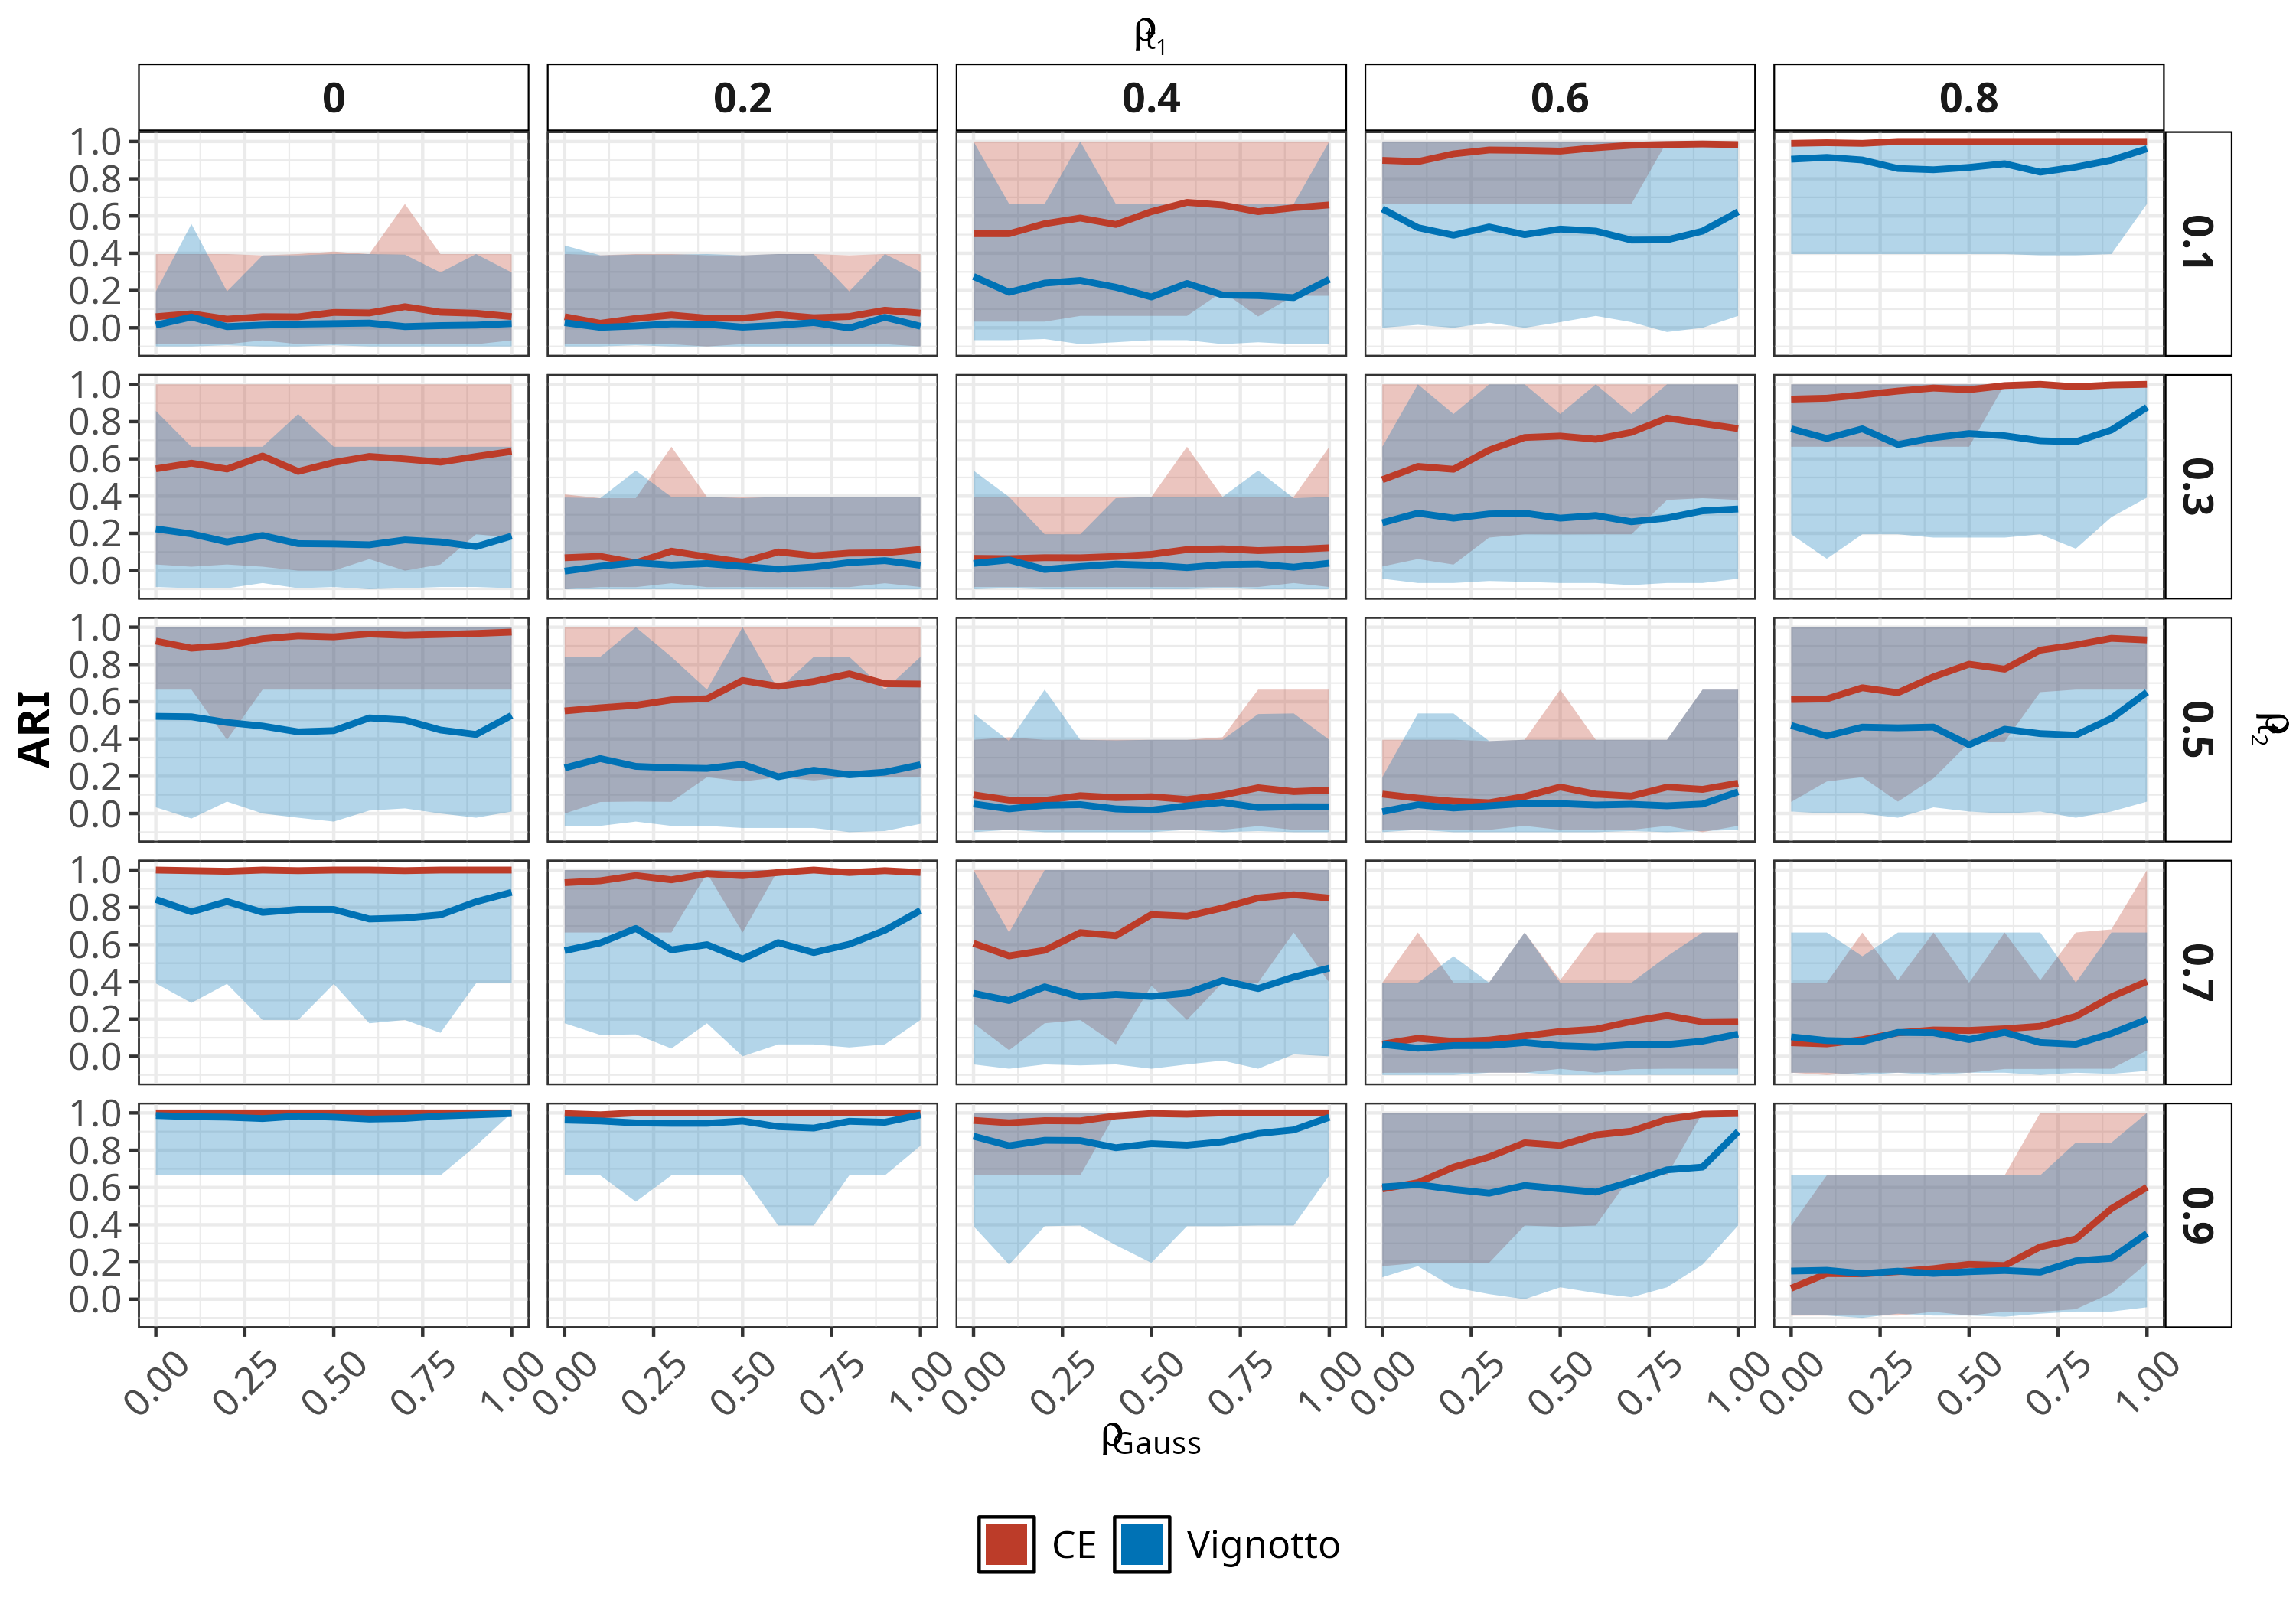
\includegraphics[width = 0.9\linewidth]{plots/sim_01b_ce_vs_vi_dqu_0.9.png}
    \caption{\emph{Comparison of clustering methods for two dimensions and two known clusters. The x-axis represents the Gaussian correlation parameter for both clusters, while the facet labels present the t-copula correlation parameters for the two known clusters the data is simulated with. The Adjusted Rand Index (ARI) is used to compare the clustering solutions. The proposed method is shown to be superior to the leading competitor in the bivariate case, \cite{Vignotto2021}. Both models perform better when the difference in the t-copula correlation parameters between the two clusters is larger, and when Gaussian correlation is higher.}}
    \label{fig:01_ce_vs_vi}
\end{figure}


\subsection{Extension to $>2$ dimensions} \label{subsec:sim_extension}

\begin{itemize}
    \item Also shown to work well for three dimensions ...
\end{itemize}

\todo{write caption}
\begin{figure}[H]
    \centering
    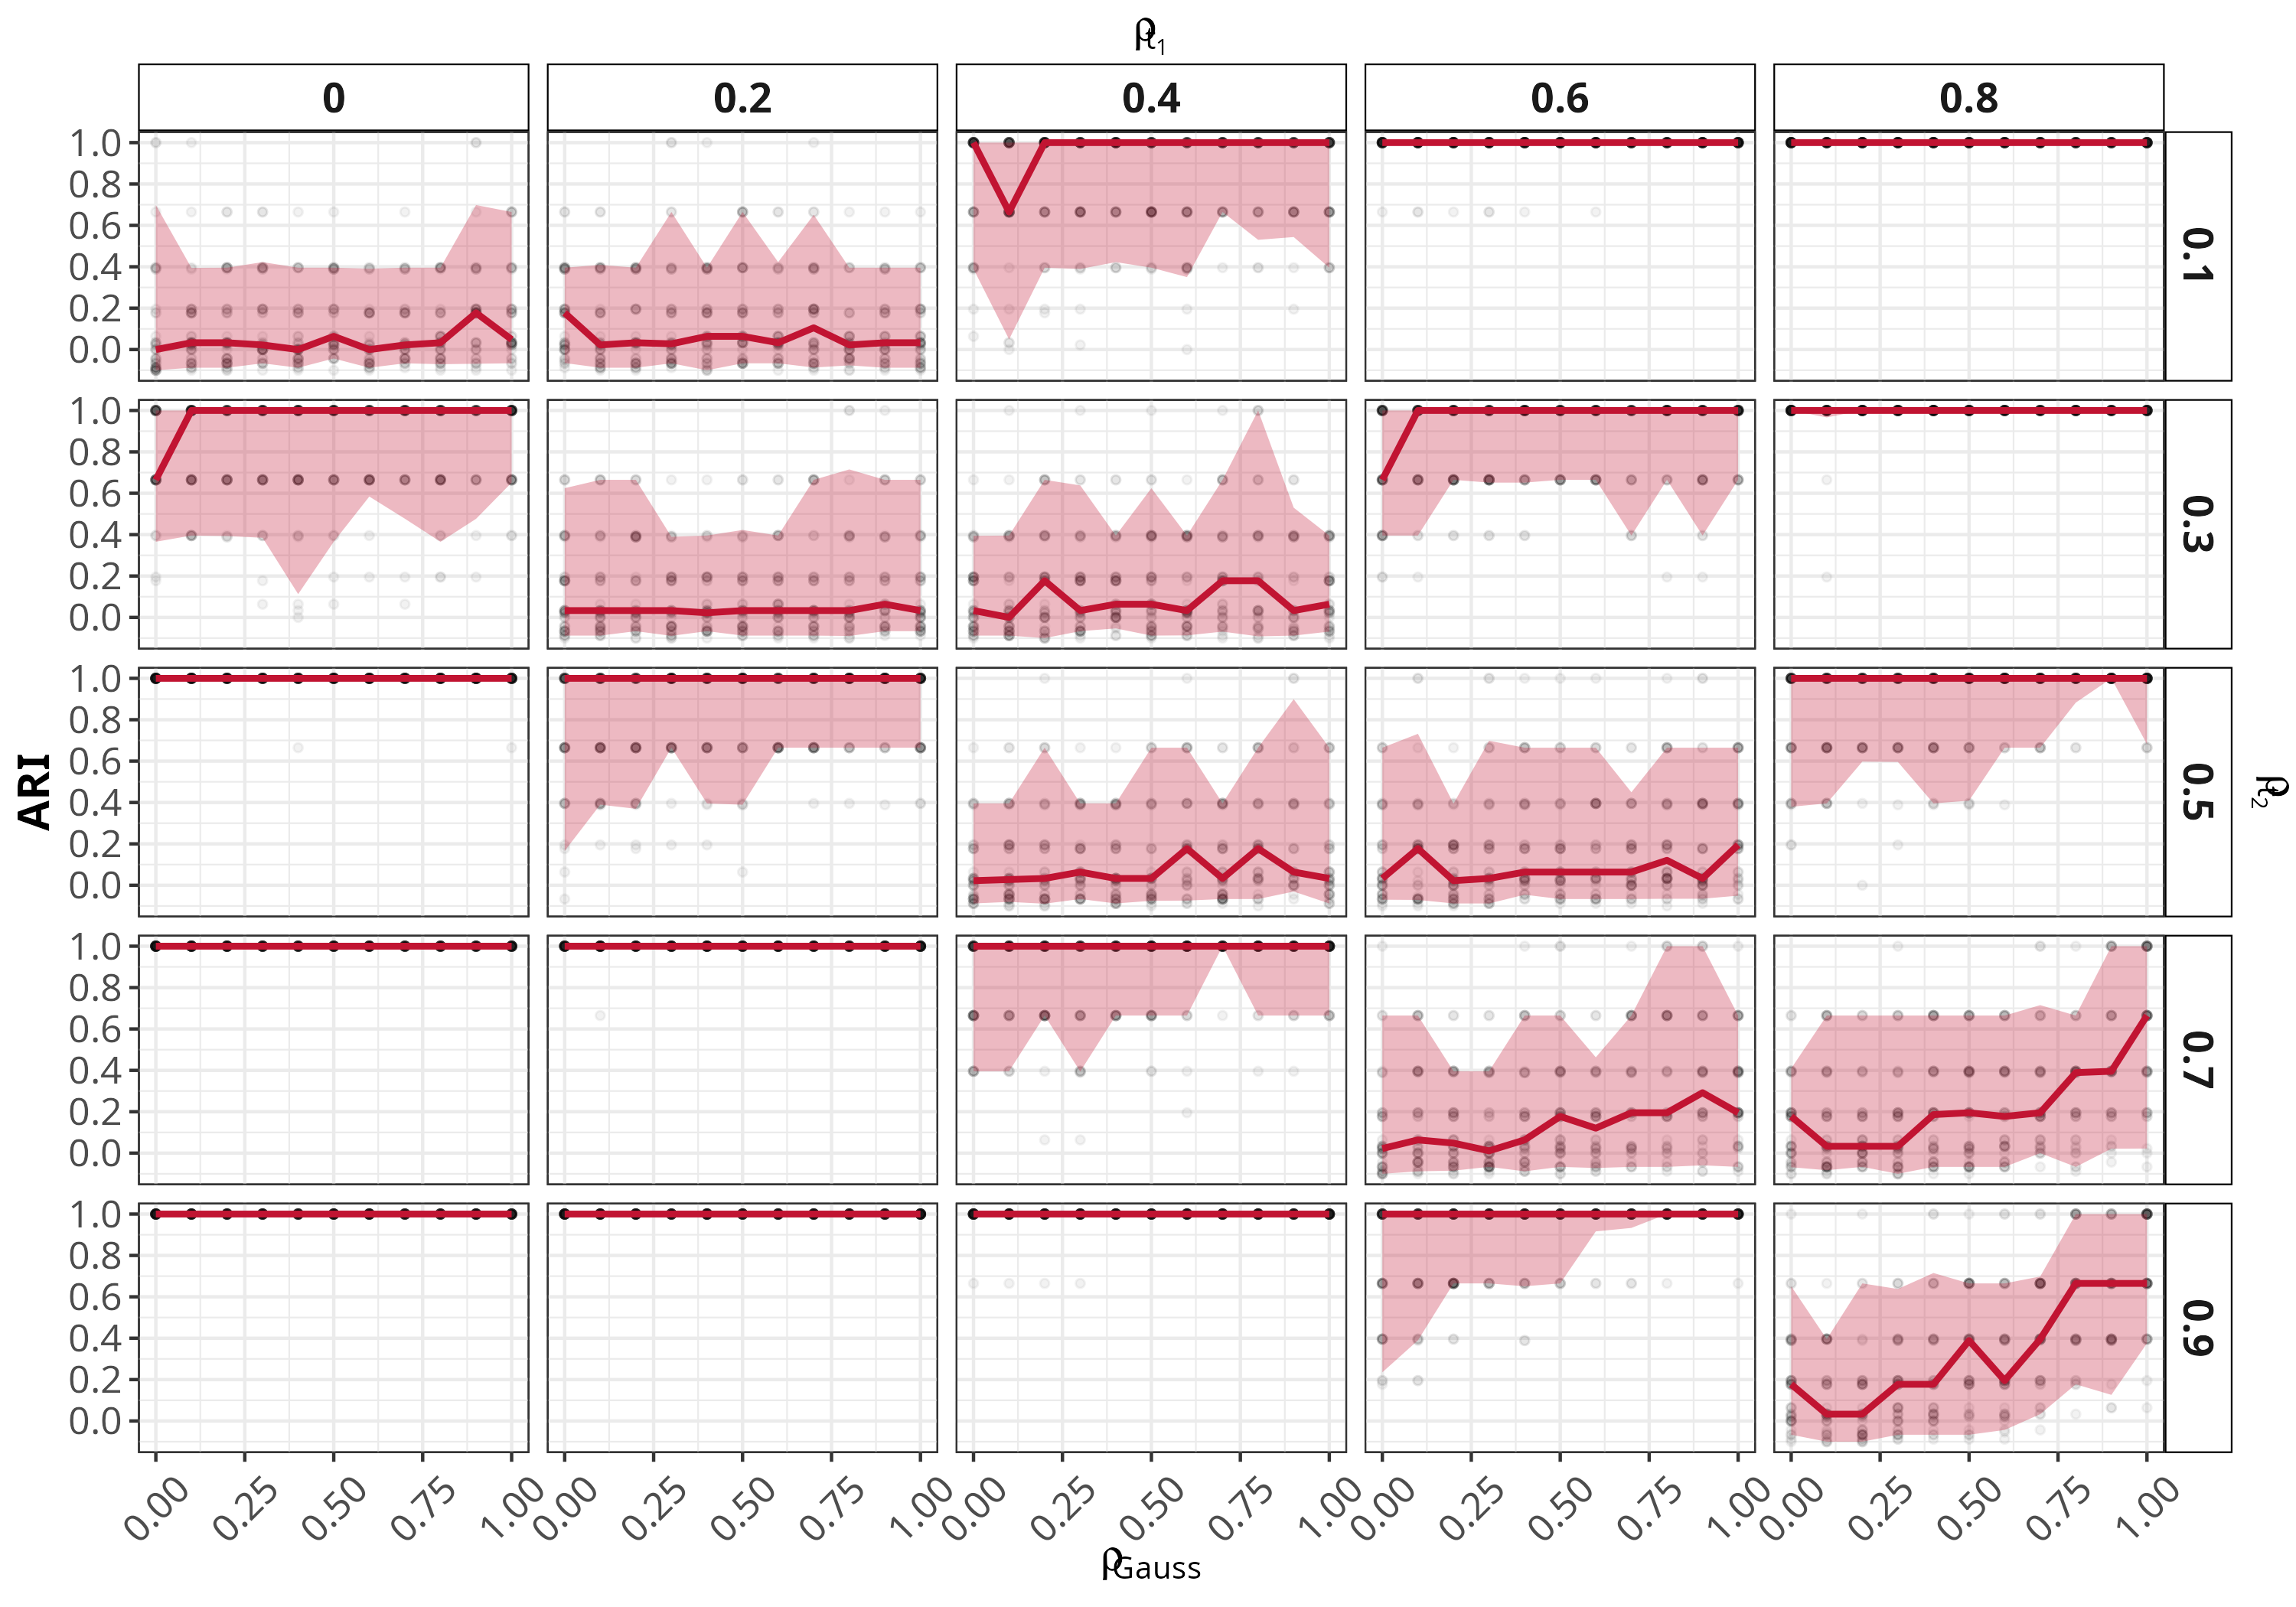
\includegraphics[width = 0.9\linewidth]{plots/sim_01c_js_sens_3_var_dqu_0.9.png}
    \caption{\emph{caption}}
    \label{fig:02_3d}
\end{figure}

\subsection{More realistic example} \label{subsec:sim_realistic}

\begin{itemize}
    \item Generated more realistic example to somewhat match the structure of the Irish dataset. 
    \item ? locations, ... \todo{fill in}
\end{itemize}

\todo{Write caption}
\begin{figure}[H]
    \centering
    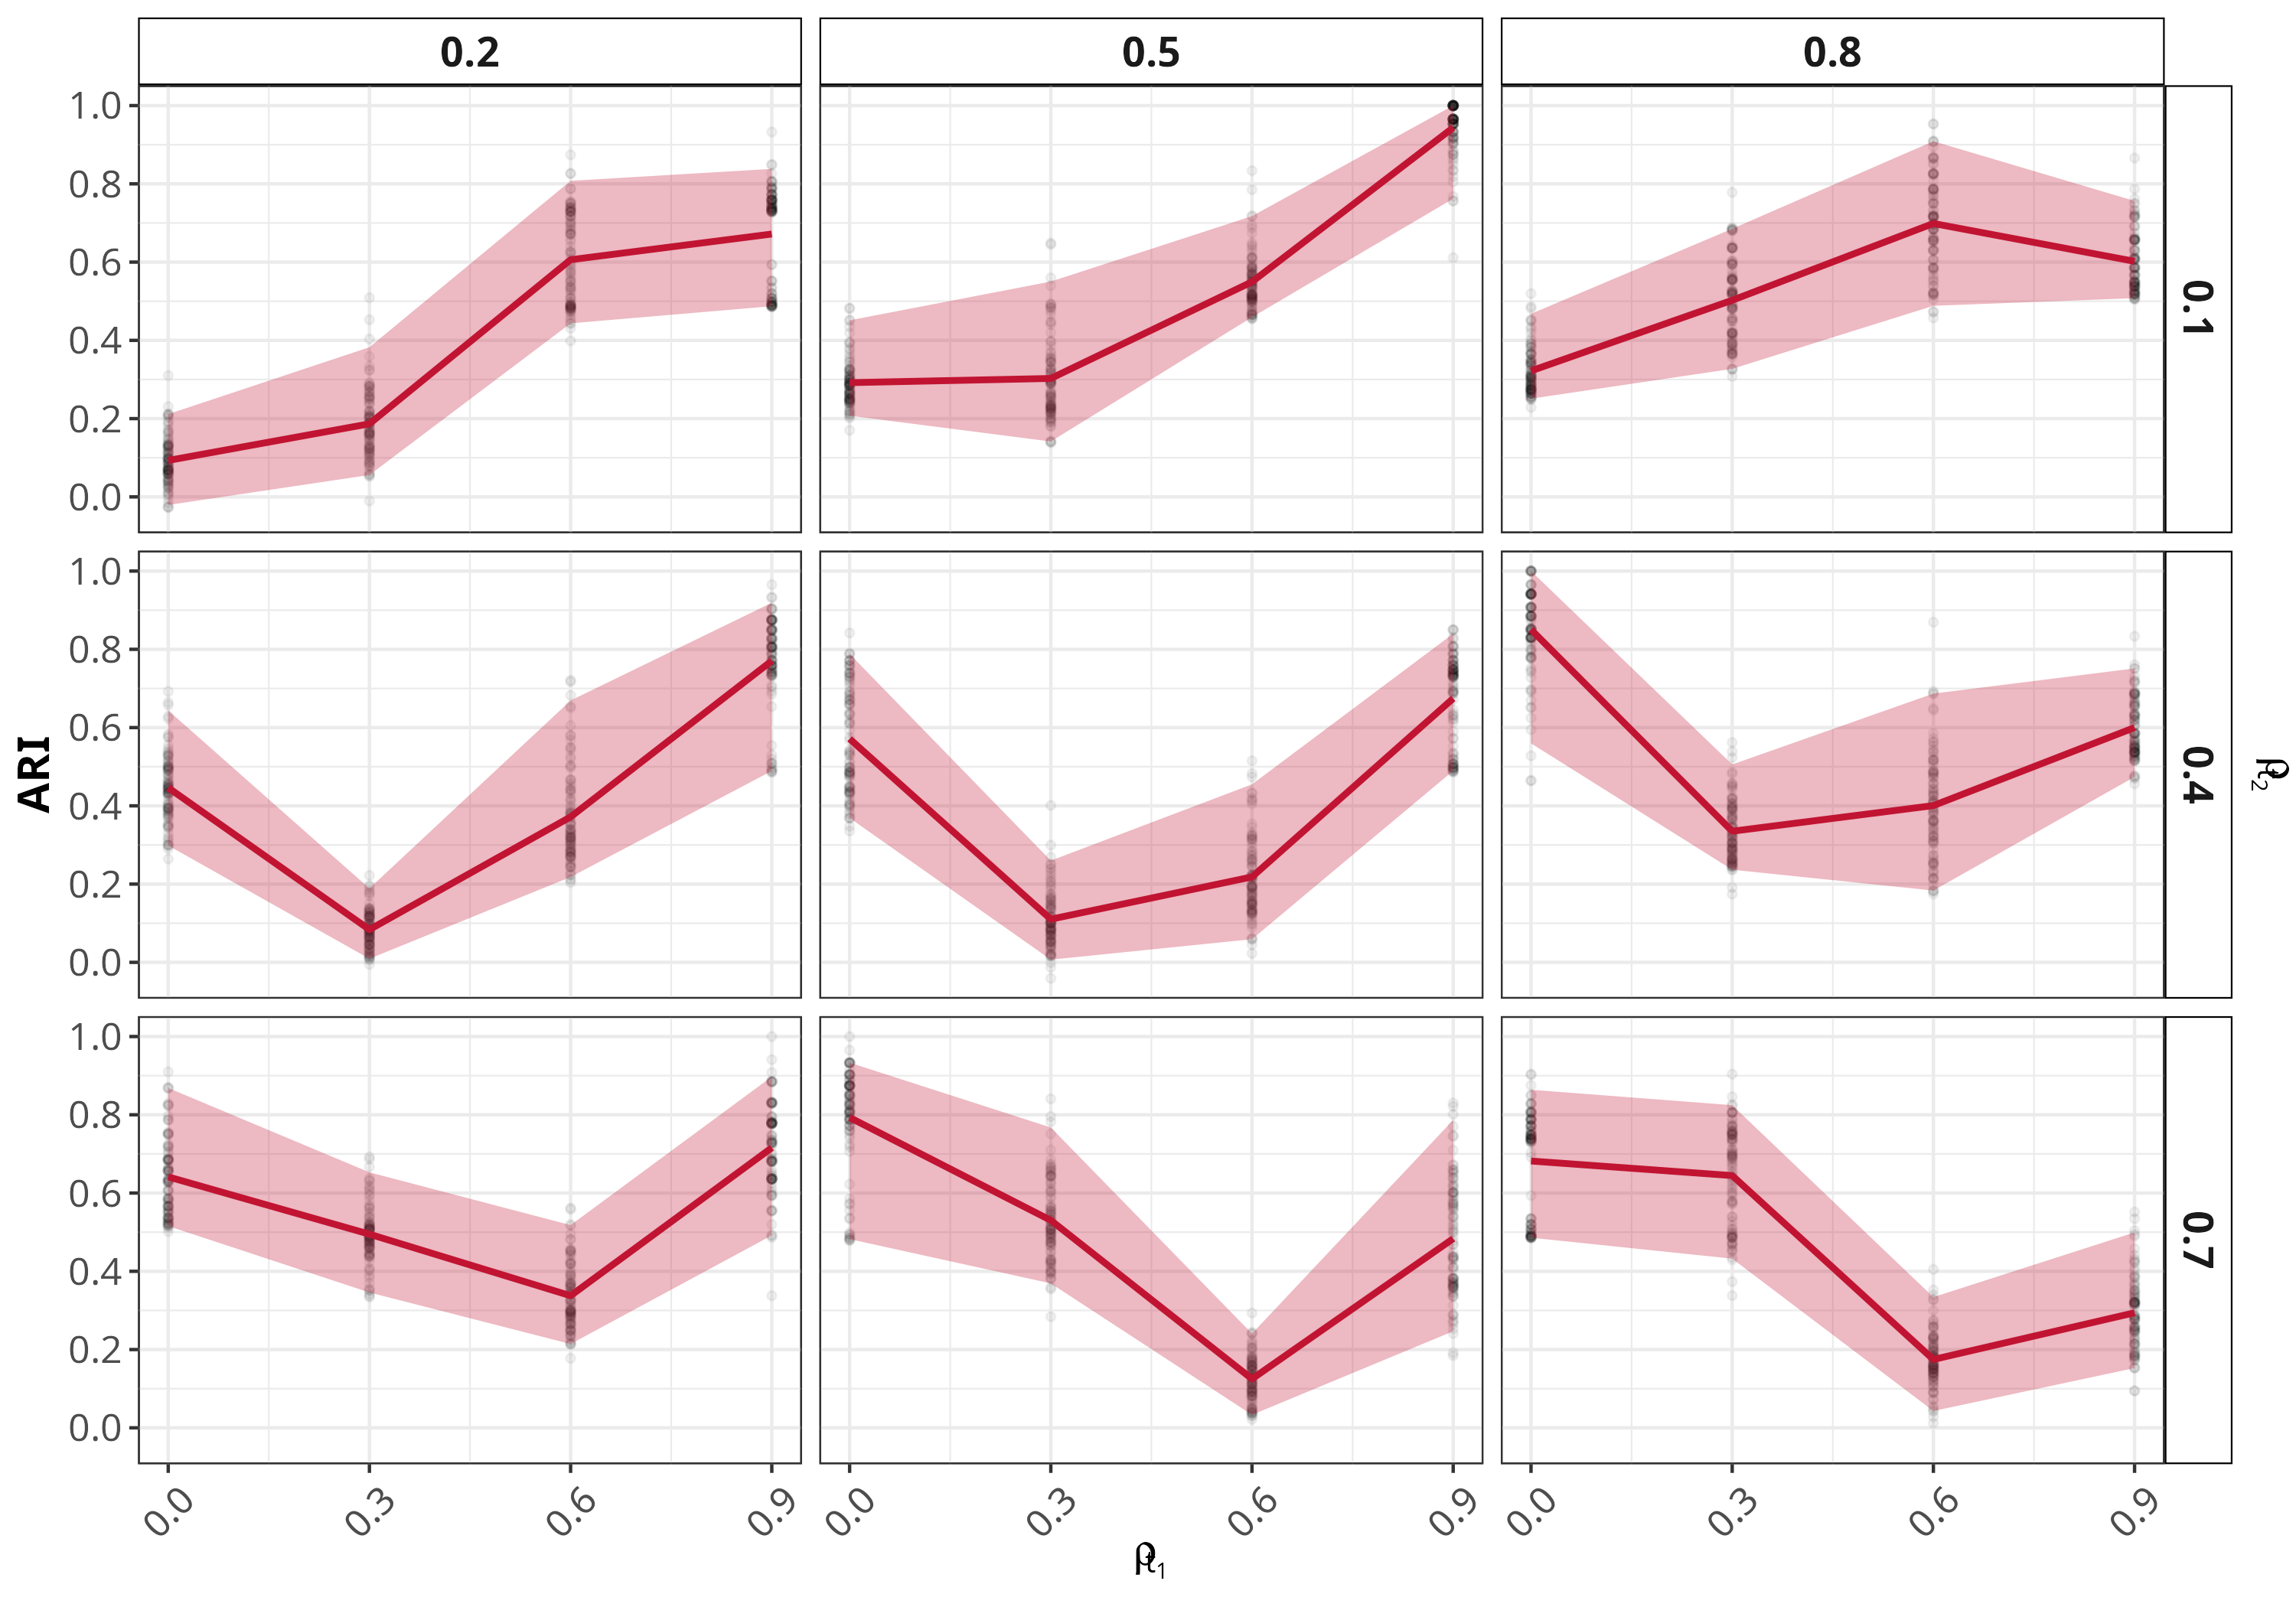
\includegraphics[width = 0.9\linewidth]{plots/sim_01d_js_sens_3_var_dqu_0.9.png}
    \caption{\emph{caption}}
    \label{fig:03_realistic}
\end{figure}



\subsection{Parameter estimation pre- and post-clustering} \label{subsec:sim_refit}

\begin{itemize}
    \item Desire to ascertain whether dependence parameters are less uncertain after clustering. 
    \item Can bootstrap using scheme in \cite{Heffernan2004} to determine uncertainty in parameter estimates. 
    \item Post clustering, can see that uncertainty is vastly reduced for both $\alpha$ and $\beta$ parameters in this simulation study. 
\end{itemize}

\subsection{Choosing the number of clusters} \label{subsec:sim_n_clust}

\begin{itemize}
    \item \todo{Describe TWGSS}
    \item \todo{Describe AIC}
\end{itemize}

\section{Applications}
\subsection{Irish meteorological data} \label{subsec:app_irl}

\begin{itemize}
    \item 
\end{itemize}

\subsection{US urban air pollution data} \label{subsec:app_us}

\begin{itemize}
    \item 
\end{itemize}

\section{Discussion}

\section*{Code availability}

\newpage
\bibliography{library}

\end{document}
